\section{Current Status}
We are currently nearing the end of the vertical slice development, which spans most of the first act of the game's story. In order to do this, we've built complex quest and dialogue systems, as well as intricate platforming and combat mechanics. The slice also features most of the main cast of characters, as well as two distinct and detailed environments.

\begin{figure}[h]
  \centering
  \begin{subfigure}[b]{0.60\textwidth}
    \centering
    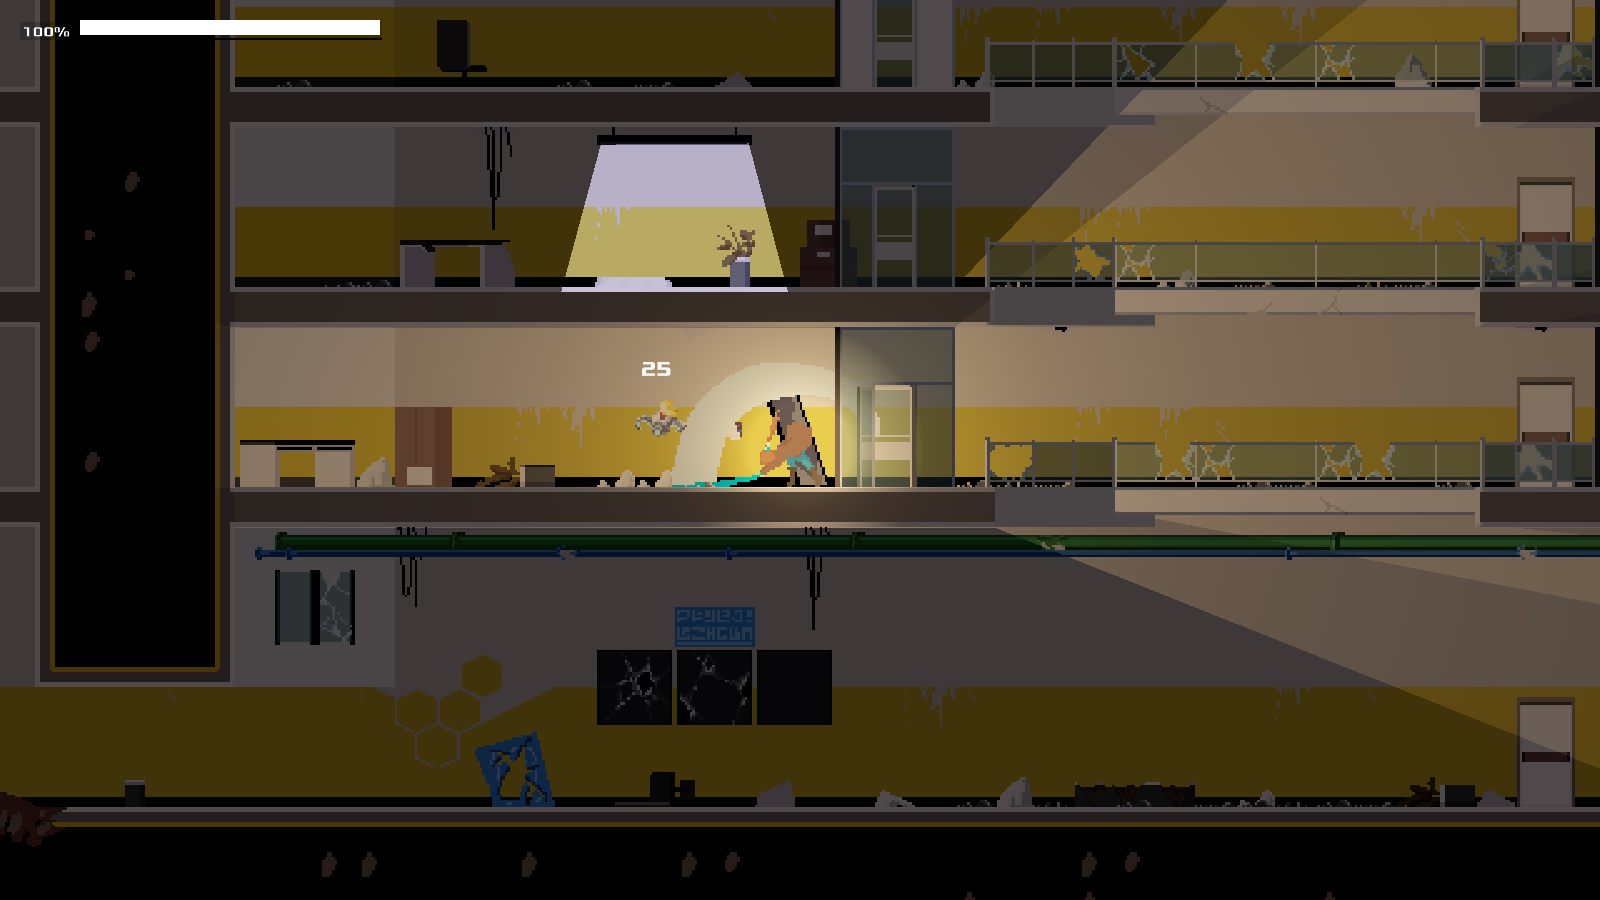
\includegraphics[width=\textwidth]{../press/screenshot 1.png}
  \end{subfigure}
  \begin{subfigure}[b]{0.35\textwidth}
    \centering
    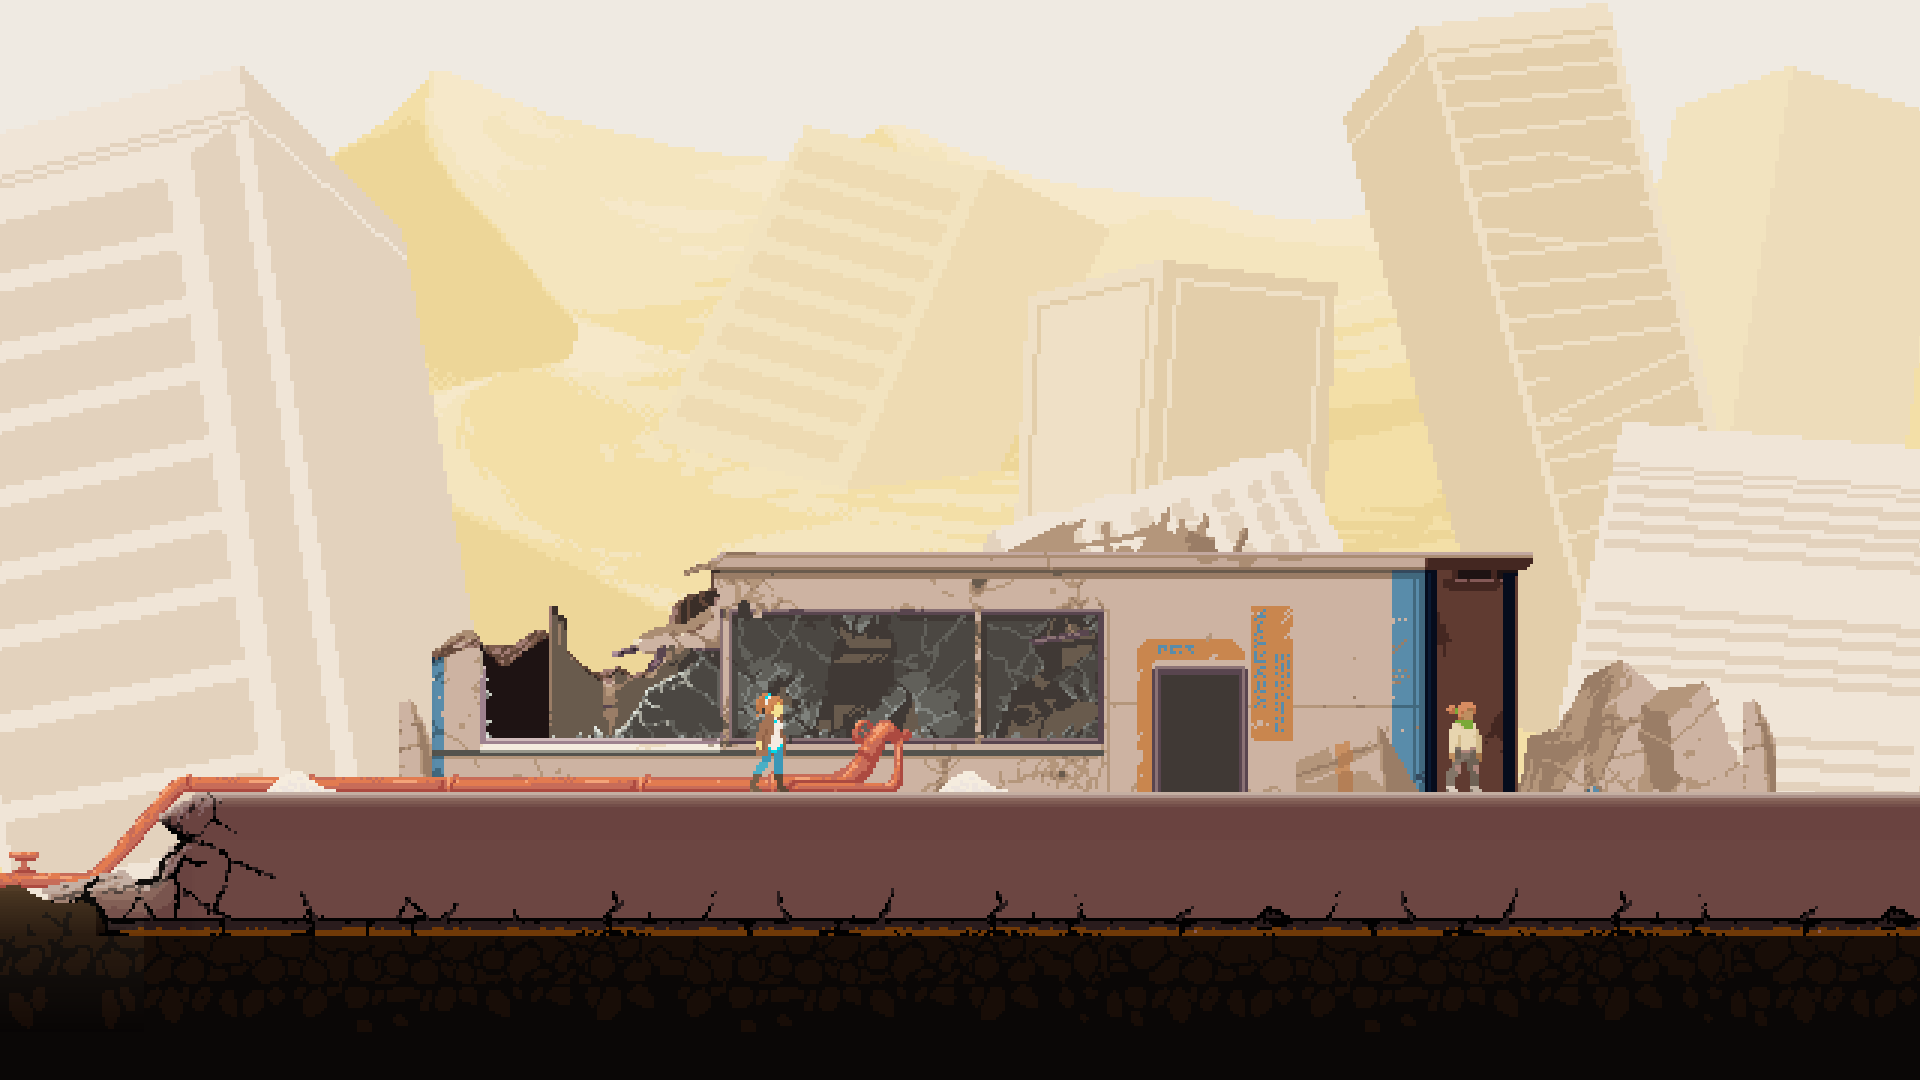
\includegraphics[width=\textwidth]{../press/screenshot 8.png}
  \end{subfigure}
  \vskip -0.5cm
  \begin{subfigure}[t]{0.35\textwidth}\vskip 0pt
    \centering
    \includegraphics[width=\textwidth]{../press/screenshot 2.png}
  \end{subfigure}
  \begin{subfigure}[t]{0.55\textwidth}\vskip 0pt
    \centering
    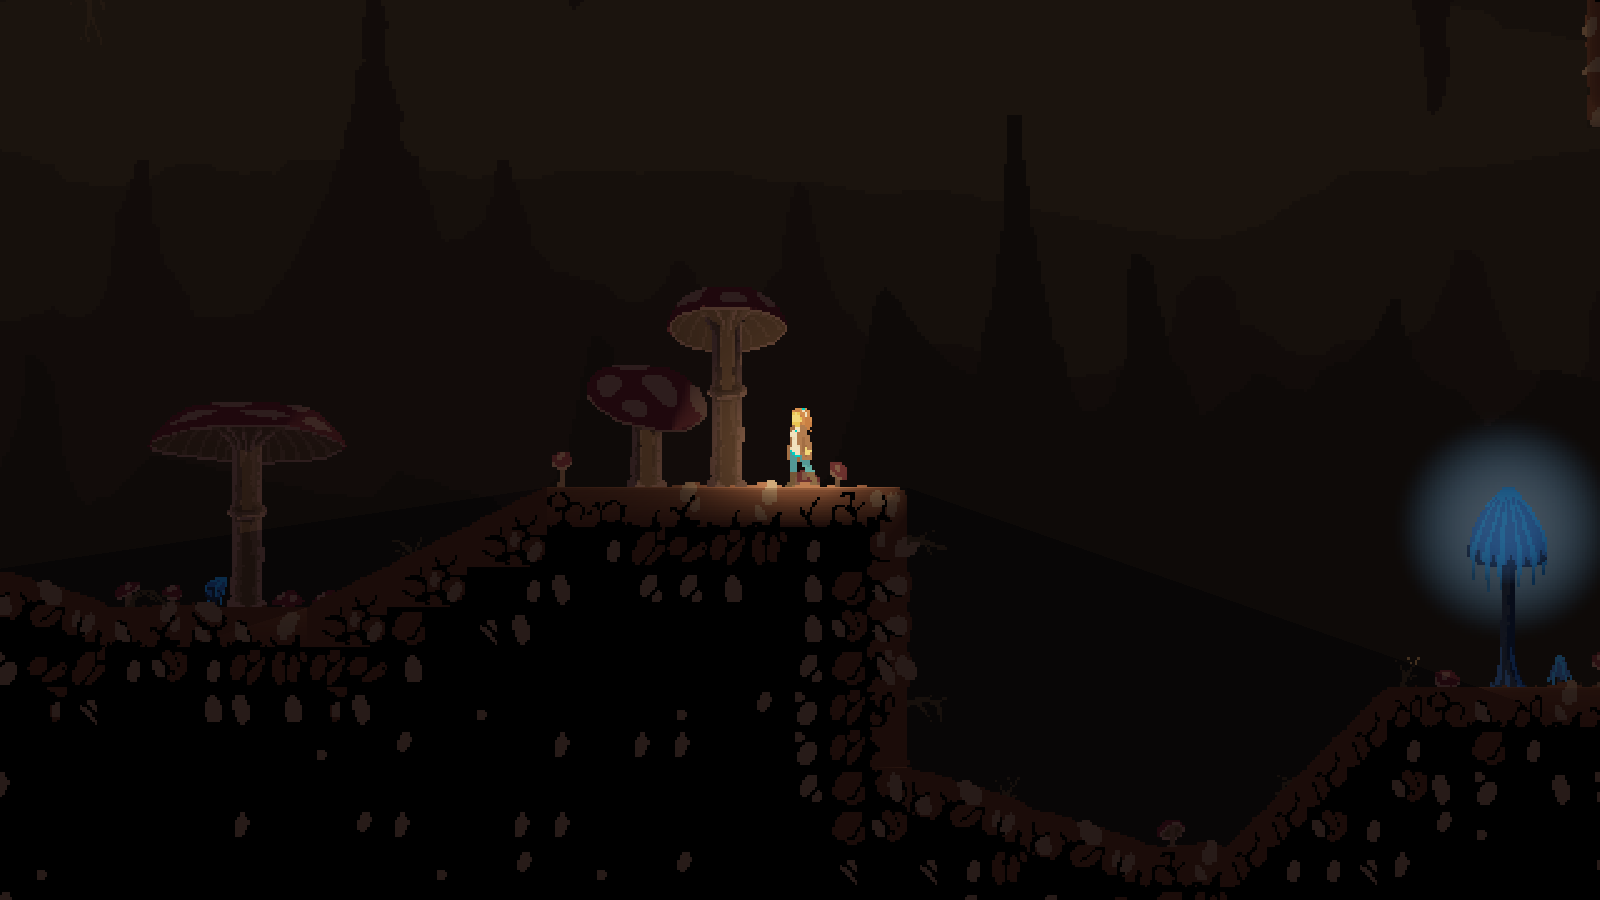
\includegraphics[width=\textwidth]{../press/screenshot 3.png}
  \end{subfigure}
\end{figure}

Having spent a good chunk of pre-production and the slice development on figuring out our process and developing our tools, we can now produce content with much more confidence and efficiency. Most of the required systems for the full game are in place and working well, too, so we can focus more on the design.

We've also written detailed design documents describing the \href{https://kandria.com/lore}{setting}, \href{https://kandria.com/plot outline}{story}, \href{https://kandria.com/characters}{characters}, \href{https://kandria.com/art}{visuals}, and so forth in order to create a cohesive narrative and world for the player to explore.

\clearpage
\subsection{Story and World}
Kandria's world is set in the not too distant future. Humanity has built massive, glistening cities on earth's surface, and deep webs of tunnels and complexes underground. Most of the manufacturing process is automated now, even down to primitive humanoid robots... or at least so you would be led to believe if you enjoy a life of comfort on the surface. Underground the situation was very different. People were used primarily as an exploited workforce, either to maintain and manage the systems used above, or to mine and process rare materials.

Around this time, true AI was finally discovered. By a process that was not fully understood, devices could be manufactured that would learn and interpret information like a real brain. It didn't take long before this technology was incorporated into a humanoid chassis, birthing the first true android. This posed another vital step in the progress of fully automating all of human civilisation. However, shortly after the first few androids were developed in the field, calamity struck.

\begin{figure}[h]
  \centering
  \includegraphics[width=\textwidth]{../press/screenshot 6.png}
\end{figure}

The surface world was almost entirely wiped out, cities flattened and ground into dust with only ruins and deserts left in their wake. Many of the underground tunnels and structures collapsed, and humanity was brought to the brink of extinction. Only few survived underground, and with the catastrophe in mind, became reclusive and protective.

\clearpage
\begin{figure}[h]
  \centering
  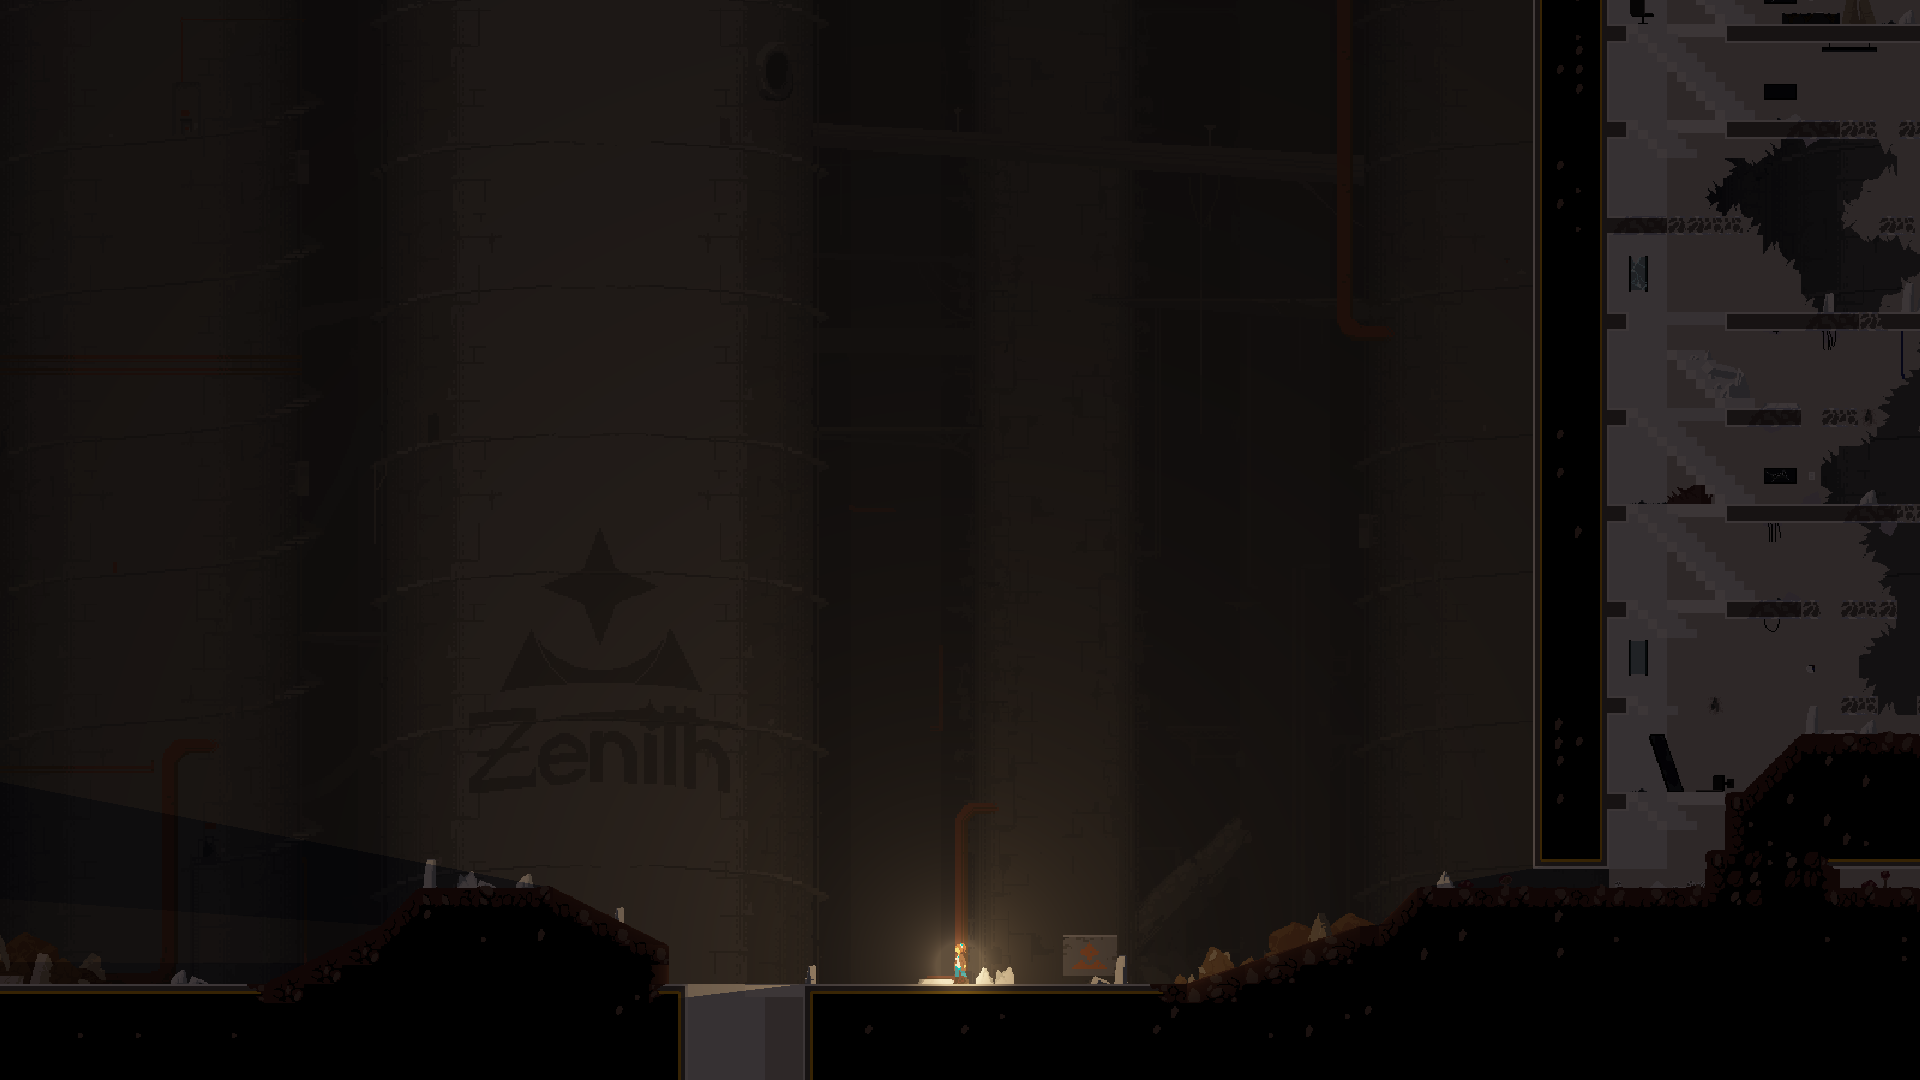
\includegraphics[width=\textwidth]{../press/screenshot 9.png}
\end{figure}

The game begins a few decades after the calamity, set in the valley of the former city of Zenith -- the underground areas now controlled by a few distinct factions, with raiders and other outcast groups roaming the tunnels and abandoned sites. One of those factions is undergoing internal conflict, a violent and militaristic group is struggling for power. Worried by this turn of events, and having discovered an old-world seed cache, Fi and her closest friends decide to separate and attempt to build their own faction back on the abandoned surface.

Near this seed cache they discover the slumbering remains of an android -- you -- and manage to reactivate it. Now back on your feet, with all of your memories lost to a data corruption, it's up to you to decide what to do. Will you follow after them or forge your own path?

Exploring the underground you'll come across other factions, each with their own values and beliefs, their own ideas on how to recover from this catastrophe. It is now up to you to earn their trust and defend what you hold dear from the harsh world. No matter what you do though, the conflict in Fi's home faction is reaching its boiling point, and will inevitably affect everyone else in the valley.

%%% Local Variables:
%%% mode: latex
%%% TeX-master: "pitch"
%%% TeX-engine: luatex
%%% End:
